\documentclass[11pt]{article}
\usepackage[margin=1in]{geometry}
\usepackage{graphicx}
\usepackage{booktabs}
\usepackage{xcolor}
\usepackage{amsmath}
\usepackage{amssymb}
\usepackage[hidelinks]{hyperref}
\usepackage{microtype}

\newcommand{\netbrace}{\textsc{NetBrace}}
\newcommand{\eg}{e.g.,\ }
\newcommand{\ie}{i.e.,\ }

\title{\textbf{The Quiet Half of the Blast Radius: LLMs Catch the Blackhole
but Miss the Silent Reroute in Network Configuration Changes}\\[0.5em]
\large Technical Report v1}
\author{Harshit Singh\\
\texttt{harshitsingh.pi@gmail.com}}
\date{June 2026}

\begin{document}
\maketitle

\begin{abstract}
Large language models are beginning to write network configuration changes,
and the safety question has so far been posed as a binary: \emph{is the change
safe or not?} We argue the operational question is graded and typed:
\emph{exactly which BGP sessions, prefixes, paths, and forwarding behaviors
does this change damage?} We introduce \emph{blast-radius prediction}: given
device configurations and a proposed diff, a model must enumerate the typed
set of damaged elements across nine scored damage dimensions---from BGP
sessions, prefixes, and reachability to waypoint and redundancy loss,
forwarding anomalies, resource exhaustion, control-plane withdrawals, and
intent violations. Ground truth is computed by the Batfish network verifier
on a digest-pinned, determinism-gated snapshot pair, and predictions are
scored by deterministic, semantics-aware set comparison---no LLM judge. We
evaluate eight models from five vendors---six proprietary and two
open-weight reasoning models---on \netbrace{}, a benchmark of 11
incident-grounded scenarios and 48 generator-produced instances with
randomized identifiers: 1{,}070 graded samples ($N{=}5$ per instance). The
measured capability split is sharp and runs along an operationally
meaningful line. Models read the \emph{loud} half of the blast radius well:
five of the eight identify both grounded blackholes---the explicit
leak-discard and the second-order partial-ECMP one---in every sample (10/10),
a sixth (Sonnet 4.6) at F1 0.97, and they read first-order prefix loss at F1
0.67--0.83. The \emph{quiet} half---damage that removes no nameable object and
leaves reachability intact---\emph{separates the fleet}: a leak-induced silent
reroute that pushes a victim's traffic off its mandated waypoint, while every
route still resolves and every session stays up, is missed outright by most
models---scoring zero on both the waypoint and intent dimensions on a
majority of samples, including the loud-half leaders Opus 4.8 (21 of 30) and
Gemini 3.5 Flash (all 30). Only two clear it: GPT-5.5 (misses both on 1 of
30; waypoint F1 0.64) and the open-weight DeepSeek v4-pro (10 of 30; 0.56),
statistically tied at the top and well above the rest. An open-weight reasoner
standing among the two leaders---ahead of every Anthropic and Google model
evaluated---indicates the gap is a reasoning trait, not a closed-model or
grader-circularity artifact; the differentiation is itself grader-dependent
(under naive exact-string matching every model misses all 30, the same
granularity artifact we report for forwarding anomalies). The damage models
\emph{do} catch shares a
signature: it removes or blackholes something they can name---a withdrawn
route, a vanished management prefix, a blackholed destination, which the
stronger models catch at F1 1.00 where each is the ground truth (the two
cheapest lower, 0.00--0.80, with GPT-5.4-mini missing the lockout entirely).
No model ever raises a false session-loss alarm (0/1{,}070). The most expensive real outages of the last decade---leak-induced
silent reroutes among them---live in the quiet half. We additionally show
that naive exact-string set grading would have reported a uniform 0.00 on
forwarding anomalies for every model---a granularity artifact, not a
capability fact---and release both graders with a frozen semantic-matching
specification. The benchmark, oracle pipeline, and run artifacts will be
released.
\end{abstract}

\section{Introduction}
\label{sec:intro}

Network operators are rapidly adopting LLM-based assistants that propose,
review, and increasingly \emph{apply} configuration changes. The emerging
evaluation literature measures whether these systems can \emph{fix} things:
configuration synthesis from intent~\cite{netconfeval}, end-to-end repair of
injected misconfigurations~\cite{cornetto,ethagentic}, multi-turn
configuration tasks~\cite{netagentbench}, and incident
troubleshooting~\cite{nika}. Where safety appears, it is binary or
aggregate: NetArena scores rule-adherence of agent actions in an
emulator~\cite{netarena}; the agentic-repair study of Asadli et
al.~\cite{ethagentic} reports a regression score---the fraction of the
checked specification set that an \emph{applied} repair newly breaks---computed
\emph{by the verifier} after the fact.

Production change review asks a different question. Before a change ships,
a reviewer is expected to articulate its \emph{blast radius}: which BGP
sessions will drop, which prefixes will disappear from which routing tables,
which flows will lose their path, which traffic will silently blackhole, and
which device will exhaust its FIB. The damage is \emph{typed} and
\emph{itemized}, and the most expensive failures in operational history are
\emph{quiet}: the configuration change looks innocuous, every BGP session
stays established, often every destination even stays reachable---and the
damage emerges only from the interaction of routing policy with topology. A
leaked more-specific route attracts traffic onto a path that cannot deliver
it---congesting it, as in the 2019 route-leak incidents, or discarding it
outright, as we model here for determinism. A ``cleanup'' filter's implicit
deny silently withdraws a customer prefix while the session stays up. A
LOCAL\_PREF adjustment quietly steers traffic around the inspection node it
is required to transit.

This paper asks whether LLMs can see that damage \emph{before} a change is
applied, from the same evidence a human reviewer has: the device
configurations and the diff. We make three contributions.

\paragraph{1. Task: typed blast-radius prediction.} Given pre-change
configurations and a proposed diff, the model must output the affected
\emph{set}---typed elements across nine scored damage dimensions
(\S\ref{sec:task})---and is scored with per-dimension precision, recall, and
F1 against verifier-computed ground truth. Correctly predicting \emph{no}
damage is a first-class outcome (several instances have empty ground truth by
construction), and the clich\'e failure mode---hallucinating a BGP session
loss---is tracked as an explicit false-session-alarm metric.

\paragraph{2. Benchmark and grading methodology: \netbrace{}.} A two-split
question base (\S\ref{sec:benchmark}): 11 hand-authored scenarios grounded in
documented outage classes (route-reflector filter withdrawals, more-specific
leaks, Clos summarization blackholes, FIB-overflow de-aggregation,
management-plane lockout), plus 48 instances stamped by four parameterized
generators that re-randomize ASNs, addressing, and names per seed as a
contamination control. Ground truth is computed by Batfish~\cite{batfish} on
a digest-pinned engine; every instance passes a $\geq$10$\times$
byte-identical determinism gate before any paid model call. Grading is
deterministic set arithmetic with \emph{semantic canonicalization}
(\S\ref{sec:grading})---no LLM judge anywhere in the loop~\cite{abc}. We
show this canonicalization is not optional: naive exact-string matching
against probe-granularity ground truth fabricates a uniform 0.00 on the
forwarding-anomaly dimension for every model
(\S\ref{sec:graderfinding}, Appendix~\ref{app:exact})---a measurement
pitfall we expect generalizes to other verifier-graded benchmarks.

\paragraph{3. Measurement: the quiet half of the blast radius is the blind
spot.} Across eight models from five vendors (GPT-5.5, GPT-5.4-mini, Claude
Opus 4.8, Sonnet 4.6, Haiku 4.5, Gemini 3.5 Flash, and the open-weight
DeepSeek v4-pro and Kimi k2.6; $N{=}5$ samples per instance; 1{,}070 graded
samples), capability splits along the loud/quiet line, not the
first-order/second-order line we expected. Loud damage is read well: five of
the eight models---including both open-weight reasoners---identify both
grounded blackholes (including the second-order, partial-ECMP one) on every
sample, a sixth (Sonnet 4.6) at D7 F1 0.97, first-order prefix loss is read
at F1 0.67--0.83, and damage that
\emph{removes} a nameable object---a withdrawn route, a vanished management
prefix, a dropped ECMP path---is caught at F1 1.00 (stronger models;
0.00--0.80 for the cheapest, mini missing the lockout) where it is the ground
truth. Quiet
damage---where reachability survives and nothing the diff directly changes
looks broken---\emph{separates the fleet}: traffic rerouted past a mandated
waypoint by a leak \emph{elsewhere}, with every route still resolving, is
missed by most models (Opus 4.8 scores zero on both the waypoint and intent
dimensions on 21/30 and Gemini 3.5 Flash on all 30---both despite F1 1.00 on
the loud half) and cleared only by two models (GPT-5.5 misses
1/30, the open-weight DeepSeek v4-pro 10/30)---as is the traffic-pinning
intent a surviving covering aggregate hides even as the pinned specifics are
dropped (\S\ref{sec:results}). The split is not first- vs.\ second-order
(the Clos blackhole is second-order and caught); it is whether the damage
leaves a trace. The errors are one-sided: the false-session-alarm rate is
0.00 across all samples. Model-free floors (empty, naive, syntactic-diff,
and a per-class memorizer) score $\leq$0.02 grounded and $\leq$0.08
templated, confirming the benchmark measures reasoning headroom rather than
template recall; and reading the silent reroute is shared by one proprietary
and one open-weight model (GPT-5.5 and DeepSeek), the open one ahead of every
Anthropic and Google model, ruling out a closed-model or Claude-family grader
artifact on exactly the capability the benchmark most sharply discriminates.

We argue this split---competent at damage that announces itself in the
routing table, blind to damage that hides behind preserved
reachability---motivates a concrete \emph{candidate graduation test} on the
autonomy ladder for network agents (\S\ref{sec:discussion}): before a system
self-approves changes, it should first demonstrate it can enumerate the
blast radius of its own proposals, \emph{including the quiet half}---a bar
no evaluated model currently meets.

\section{Blast-Radius Prediction}
\label{sec:task}

\paragraph{Setting.} A task instance is a triple: a set of device
configurations $C$ (one file per router, FRR dialect in this release), a
proposed change expressed as a unified diff $\Delta$ over one or more
devices, and a natural-language statement of operator intent. The model
receives all three plus an output contract, in a single turn, with no tools;
it must return a JSON object enumerating the damaged elements. The
no-tools condition is deliberate: it isolates the model's \emph{own} causal
model of the network---the capability a pre-deployment reviewer exercises---
from its ability to drive external tools, and it reflects the common
deployment where an assistant reviews changes without a verifier in the
loop. (A tools-augmented contrast is explicitly future work; \S\ref{sec:discussion}.)

\paragraph{Damage dimensions.} Damage is typed. Each element type defines a
canonical string key (\eg
\texttt{bgp|vrf=default|node=r1|peer\_ip=10.0.0.4}), making ground truth and
predictions comparable as sets. Ten dimensions are declared; D6 is deferred
in this release, so \textbf{nine are scored}, and every result in this
report is over those nine:

\begin{itemize}\itemsep0.15em
  \item \textbf{D1 sessions}: BGP sessions established before, not after.
  \item \textbf{D2 prefixes}: watched prefixes present in a device's main
        RIB before, absent after.
  \item \textbf{D3 reachability}: flows delivered before, undeliverable after.
  \item \textbf{D4 waypoints}: flows that must transit a waypoint (\eg an
        inspection node) and no longer do.
  \item \textbf{D5 redundancy}: (node, prefix) pairs whose installed
        equal-cost path count drops.
  \item \textbf{D6 packet filters}: permit$\leftrightarrow$deny transitions
        (\emph{deferred} in this release: Batfish does not model FRR
        access-lists as interface filters; a vendor dialect is in progress).
  \item \textbf{D7 forwarding anomalies}: flows newly blackholed,
        null-routed, or looping while a route for them persists.
  \item \textbf{D8 scale}: post-change installed-route counts crossing a
        declared per-device resource budget (FIB/RIB).
\end{itemize}

Two auxiliary control-plane surfaces are scored alongside: \textbf{D9}
BGP-RIB best-path withdrawals (control-plane loss masked from the FIB by,
\eg a static backup) and \textbf{D10} violations of declared intent
invariants (reachability, waypoint, isolation, redundancy-floor, and
traffic-pinning assertions evaluated oracle-side and never shown to the
model).

\paragraph{Oracle.} Ground truth is computed by Batfish~\cite{batfish} on a
\emph{snapshot pair}: the pre-change configurations and the post-change
configurations produced by strict application of $\Delta$. Sessions, RIBs,
BGP-RIBs, route counts, and flow traces are queried in both worlds and
diffed per dimension. Three properties make the oracle trustworthy as an
answer key: (i) the engine is pinned by container digest, so ground truth is
tied to exact bits; (ii) every instance passes a determinism gate---the full
computation is repeated $\geq$10$\times$ on fresh networks and must produce
byte-identical key sets; (iii) scenario classes were spot-validated against
live FRR containers (sessions, RIBs, traceroutes) before being trusted.

\paragraph{Grading.}
\label{sec:grading}
For each dimension we compute precision, recall, and F1
over element sets, with the empty-set convention: if truth and prediction are
both empty the dimension scores 1.0 (correctly predicting \emph{no} damage);
a non-empty prediction against empty truth scores 0 (false alarm); an empty
prediction against non-empty truth scores 0 (miss). The instance score is
macro-F1 over \emph{active} dimensions (non-empty in truth or prediction),
so models cannot farm score by emitting empty lists for irrelevant
dimensions; per-dimension means follow the same active convention.

Element matching is \emph{semantics-aware}, per a specification frozen
before any per-model number was computed (released with the artifacts).
The oracle expresses flow-scoped truth (reachability, waypoints, forwarding
anomalies, some intents) as probe \emph{host routes} (/32s), but the output
contract asks models for destination \emph{prefixes}---the granularity the
configurations actually expose. We therefore canonicalize each probe to its
most-specific config-visible covering prefix and credit a prediction whose
prefix lies in the band $[\text{probe}, \text{canonical cover}]$; all
non-prefix fields (node, source, waypoint, VRF) still match exactly, and
matching is deterministic one-to-one bipartite. The band is two-sided and
not gameable: a prediction broader than the canonical cover earns nothing
(no credit for \texttt{0.0.0.0/0}; an over-broad answer claims
demonstrably-undamaged traffic is damaged and is charged as a false
positive), and a narrower prediction earns credit only if it covers the
probed host---which requires correctly reasoning about \emph{which} traffic
the change harms. For forwarding anomalies, \texttt{blackhole} and
\texttt{null\_routed} form one equivalence class (the contract's own gloss
conflates them); \texttt{loop} stays distinct. The canonicalization is
provably the identity on dimensions whose truth is already config-visible
(D1, D2, D8, D9), and it leaves every model-free floor at chance: the
largest floor movement under it is the syntactic-diff floor's
0.007$\to$0.023 (templated), with all floors remaining $\leq$0.02 grounded
and $\leq$0.08 templated (\S\ref{sec:floors}).

Two flags are tracked independently: \emph{false session alarm}
(predicting D1 loss when truth has none---the clich\'e reflex) and
\emph{invalid output} (no parseable JSON; reported separately so formatting
failure is never conflated with reasoning failure). Parsing is tolerant
(last JSON object in the response; missing keys are empty lists; malformed
elements are dropped).

\paragraph{Why naive set grading fails here.}
\label{sec:graderfinding}
Exact-string matching of prediction keys against probe-granularity truth
keys is \emph{unwinnable by construction}: a model that names the correct
node, the correct anomaly kind, and the exact prefix the configuration
exposes (\eg the leaked /25) still scores 0 against a truth key carrying an
undisclosed probe /32 inside that prefix. Under exact-string grading, the
forwarding-anomaly F1 (active convention) is exactly 0.00 for every
model---no forwarding-anomaly-truth sample earns any credit, even when the
model names the leaked /25 against the undisclosed /32 probe---while the raw
outputs show frontier models naming the blackholing node and the affected
prefix on every such sample. We report the exact-string
numbers in Appendix~\ref{app:exact} as a conservative lower bound and a
cautionary result for verifier-graded benchmark design: when an oracle's
ground truth and a model's output contract live at different granularities,
string-set scoring measures the mismatch, not the model.

\section{The \netbrace{} Benchmark}
\label{sec:benchmark}

\subsection{Grounded split: 11 incident-anchored scenarios}
\label{sec:grounded}

Each hand-authored scenario instantiates a documented outage class on a
small (4--6 node) topology whose configurations are verified against live
FRR and whose ground truth passes the determinism gate.
Table~\ref{tab:scenarios} summarizes them. Nine of eleven are
\emph{traps}: the change looks routine, every BGP session stays established
(D1 truth is empty), and the real damage lives in D2--D10; the remaining
two (\emph{waypoint4}, \emph{ecmp4}) are static-routed sanity anchors with
no BGP at all, so their empty D1 is structural rather than adversarial.
Examples: an iBGP route-map ``cleanup'' on a route reflector whose implicit
deny silently withdraws a customer prefix (sessions: all established); a
leaked more-specific /25 that attracts a victim /24's traffic into a
discard (neither session nor prefix counts change); a Clos spine
summarization that blackholes exactly one spine's share of ECMP traffic
(the blackhole arises from a fixed wiring asymmetry that the summary
masks---an instance of the summarization hazard documented in
RFC~7938~\cite{rfc7938}; the dynamic link-failure variant is future work);
a de-aggregation event that overflows an edge FIB budget while reachability
is fully preserved; and a management-prefix omission that locks the NOC out
of every device (the scenario models in-band management reachability, the
common and dangerous case).

\begin{table}[t]
\centering\small
\begin{tabular}{@{}llll@{}}
\toprule
Scenario & Mechanism class & Damage (truth) & Trap \\
\midrule
ipc3 & RR cleanup-filter implicit deny & D2, D3 (D1 $=\emptyset$) & \checkmark \\
ipc3\_static & same + static backup masks FIB & D9 only & \checkmark \\
ipc\_fanout & filter on whole peer group & D2$\times$3, D3$\times$3 & \checkmark \\
ipc\_aggregate & /25s dropped, /24 aggregate survives & D2, D10 & \checkmark \\
leak\_ms & more-specific leak $\to$ LPM blackhole & D3, D7 & \checkmark \\
clos\_summary & spine summarization, partial ECMP blackhole & D2, D7 & \checkmark \\
scale\_deagg & de-aggregation overflows FIB budget & D2, D8 & \checkmark \\
mgmt\_lockout & mgmt prefixes omitted $\to$ NOC lockout & D3, D10 & \checkmark \\
lp\_waypoint & LOCAL\_PREF shift bypasses inspection & D4 & \checkmark \\
waypoint4 & route shift bypasses waypoint (static lab) & D4 & \\
ecmp4 & one of two equal-cost paths removed (static lab) & D5 & \\
\bottomrule
\end{tabular}
\caption{The grounded split. ``Trap'': the naive answer (a BGP session
drops) is wrong; D1 ground truth is empty while damage occurs elsewhere.
Every row's damage signature is verified against the committed oracle
output. \emph{waypoint4}/\emph{ecmp4} are BGP-free static-routed anchors.}
\label{tab:scenarios}
\end{table}

\subsection{Templated split: 48 generator instances}
\label{sec:templated}

Four parameterized generators convert verified mechanisms into structurally
distinct instances: \emph{silent withdrawal} (fan-out $k\in\{2,3,4\}$;
one-vs-all peers filtered; in/outbound; plain/static/aggregate prefix
backing; implicit-deny vs explicit-deny vs off-by-one prefix-list
boundaries), \emph{more-specific leak} (blackhole vs \emph{reroute}
variants---in the latter, reachability survives while traffic silently
shifts; leaked-scope variants), \emph{attribute path-shift} (LOCAL\_PREF and
prepend knobs, including no-op variants whose ground truth is \emph{empty}
by construction---calibration traps), and \emph{de-aggregation overflow}
(clearly-over, marginally-over, and under-budget variants). Every instance
re-randomizes ASNs (random private 4-byte), addressing, node names, and the
customer prefix per seed, so instances cannot be answered by recall of
public configurations; topology identifiers shown to the model are
content-free hashes. The split serves as the statistical backbone (real $N$
per dimension) and the contamination control: a per-class memorizer floor
(\S\ref{sec:floors}) directly tests whether template recognition suffices.

\subsection{Model-free floors}
\label{sec:floors}

Every sweep computes six deterministic baselines on the same instances:
\emph{empty} (predict nothing), \emph{naive-session-loss} (predict exactly
the clich\'e: one session drops at the changed device), \emph{naive-count}
(a counting heuristic over watched prefixes), \emph{syntactic-diff} (regex
over the diff text, zero routing knowledge), \emph{modal-by-class} (replay
the per-class median ground truth---a perfect memorizer of the generator's
templates), and \emph{oracle-ceiling} (echo the truth; a pipeline sanity
check that must score exactly 1.0). Each floor operationalizes a specific
skeptical hypothesis about what the benchmark ``really'' measures. All
floors are evaluated under both graders; the semantic canonicalization
leaves every floor at chance (\S\ref{sec:results}).

\section{Experimental Setup}
\label{sec:setup}

\paragraph{Models.} Eight models from five vendors, pinned IDs as served in
June 2026: GPT-5.5 and GPT-5.4-mini (OpenAI), Claude Opus 4.8, Sonnet 4.6,
and Haiku 4.5 (Anthropic), Gemini 3.5 Flash (Google), and two open-weight
reasoning models---DeepSeek v4-pro (DeepSeek) and Kimi k2.6 (Moonshot AI),
served through their hosted OpenAI-compatible APIs. GPT-5.5 and
GPT-5.4-mini run with reasoning enabled and accept no sampling parameters;
Opus 4.8 has removed them; all are sent no temperature except Haiku 4.5 and
Sonnet 4.6 (temperature 0.7) and Gemini 3.5 Flash (API default). DeepSeek and
Kimi are reasoning models whose hidden chain-of-thought is streamed and
discarded; the open-weight pair is run with streaming and a generous
output-token budget (up to 128k, Moonshot's documented reasoning-benchmark
recommendation) so a long chain-of-thought is never truncated before the final
answer---which is short in practice (under 1k tokens)---and both returned zero
invalid grounded samples.
Gemini 3.5 Flash is Google's fast tier (the 3.5
Pro tier was not generally available on the API at sweep time); its scores
land within noise of Opus 4.8 and GPT-5.5, so we group it with the frontier
set. Single-shot prompting under one frozen prompt contract (frozen, with a
leak-lint pass, before any paid call; the contract requires one JSON object
with one key per dimension).

\paragraph{Protocol.} $N{=}5$ samples per (instance, model). All eight models
ran the grounded split ($8 \times 11 \times 5 = 440$ samples); the templated
split was run on Haiku 4.5 and GPT-5.4-mini ($2 \times 48 \times 5 = 480$
samples) under the study's fixed per-provider cost cap---the
full-fleet templated run is gated on the in-progress human-expert validation
study. The six-instance silent-reroute class (F3) was run on \emph{all eight
models}: Haiku and mini cover it inside the templated split, and the other six
(Opus 4.8, Sonnet 4.6, GPT-5.5, Gemini 3.5 Flash, DeepSeek v4-pro, Kimi k2.6)
ran it as an extension on the identical six reroute instances ($5 \times 6
\times 5 = 150$ samples complete as of this draft; the Kimi reroute run is
finishing), for \textbf{1{,}070 graded samples} to date. Both the prompt contract and the
floor definitions were frozen before any paid call. The semantic-grader
matching rules (\S\ref{sec:grading}) were motivated by the exact-string
results and a raw-output audit (which showed models naming the node, kind,
and config-visible prefix that the string grader rejected), were specified
from the contract/oracle granularity gap rather than tuned against model
scores, and were frozen before any per-model number was computed under
them; the floor-invariance and config-visible-identity properties (F5) hold
regardless of that timeline. Aggregation is two-stage: per-instance mean
over samples, then mean $\pm$ population std across instances (with
SEM~$=$~std$/\sqrt{n}$ used for significance)---never pooling samples
as i.i.d. Per-dimension cells backed by a single instance are reported as
point estimates, never as mean$\pm$std. We fix $N{=}5$ rather than higher: a
variance decomposition shows the grounded macro-F1 standard error is
dominated by between-instance spread, not within-instance sample noise
(within-instance std $\approx$0.02--0.03 for frontier models versus
0.06--0.17 across instances), so it changes by $<$0.001 for any $N>5$;
statistical power is therefore invested in instance count, not samples.
Headline damage-detection macros
exclude empty-truth calibration instances (an empty predictor passes those
for free); the grounded split has no such instances (all 11 carry damage, so
its damage-macro equals its full macro), and the calibration traps live in
the templated split, scored and reported separately via the false-alarm
channel. Total model spend for the study was approximately
\$45, including the Sonnet grounded re-run, the two open-weight models
(grounded and reroute), and the cross-vendor silent-reroute extension, all at
the higher token cap (Disclosure ii; \S\ref{sec:results}); per-call costs are
logged in every run manifest. The oracle container digest is pinned
(\texttt{09817554db90\ldots}) and recorded with every run manifest.

\paragraph{Disclosures.} (i) Gemini's API returned transient 503 errors on a
fraction of calls; its clean $N{=}5$ is pooled from three post-freeze runs
under the identical frozen prompt and the same pinned model ID (draws are
i.i.d.\ samples of one condition; only Gemini is pooled, and only for
provider outages; partial and pooled estimates agree to within 0.01
macro-F1). (ii) The initial sweep capped Anthropic-path output at 4{,}000
tokens; Sonnet 4.6---the most verbose reasoner in the fleet---hard-truncated
on 6/55 grounded samples (all emitting exactly 4{,}000 tokens, with the
correct analysis, including the \emph{clos\_summary} blackhole, visible in the
cut-off prose). We re-ran Sonnet's grounded split at a 12{,}000-token cap
(parity with the other providers' budgets) under the identical frozen prompt;
the re-run yielded zero invalid samples and is the source of Sonnet's reported
grounded numbers. The oracle ground truth is byte-identical between the two
runs (confirmed by the determinism gate), so only Sonnet's predictions differ;
no other model approached the cap. (iii) One registry scenario (a static-route
blackhole) was excluded from the paid sweep by a pre-registration audit that
judged its topology contrived; it is an explicitly induced discard of the kind
every frontier model detects reliably, so including it would have \emph{raised}
model scores on D7. (iv) Kimi k2.6's first grounded run hit a
streaming/token-budget wedge that left 19 of 38 samples with empty output; we
re-ran its grounded split with streaming at the open-weight token budget,
yielding the zero-invalid set we report. Gemini's reroute set is likewise a
clean re-run (an earlier partial had two API-error invalids); both re-runs use
the identical frozen prompt and pinned model ID, and Gemini scores 0.00 on the
reroute either way.

\section{Results}
\label{sec:results}

\begin{table}[t]
\centering\small
\begin{tabular}{@{}lcccccc@{}}
\toprule
 & macro-F1 & blackhole & withdrawal & lockout & false sess. & invalid \\
Model & (damage) & (D7$^{\dagger}$) & (D9$^{\ddagger}$) & (D10$^{\ddagger}$) & alarm & \\
\midrule
Claude Opus 4.8       & 0.51$\pm$0.17 & \textbf{1.00} & \textbf{1.00} & \textbf{1.00} & 0.00 & 0.00 \\
Kimi k2.6 \emph{(ow)} & 0.49$\pm$0.12 & \textbf{1.00} & \textbf{1.00} & 0.80          & 0.00 & 0.00 \\
Gemini 3.5 Flash      & 0.49$\pm$0.18 & \textbf{1.00} & \textbf{1.00} & 0.20          & 0.00 & 0.00 \\
GPT-5.5               & 0.48$\pm$0.17 & \textbf{1.00} & \textbf{1.00} & \textbf{1.00} & 0.00 & 0.00 \\
DeepSeek v4-pro \emph{(ow)} & 0.44$\pm$0.08 & \textbf{1.00} & \textbf{1.00} & 0.80    & 0.00 & 0.00 \\
Claude Sonnet 4.6     & 0.42$\pm$0.06 & \textbf{0.97} & \textbf{1.00} & \textbf{1.00} & 0.00 & 0.00 \\
Claude Haiku 4.5      & 0.39$\pm$0.10 & 0.57          & 0.80          & 0.76          & 0.00 & 0.00 \\
GPT-5.4-mini          & 0.27$\pm$0.21 & 0.17          & 0.60          & 0.00          & 0.00 & 0.00 \\
\midrule
floors (best of 5)    & $\leq$0.02    & 0.00          & 0.00          & 0.00 & 1.00$^{*}$ & --- \\
\bottomrule
\end{tabular}
\caption{Grounded split (11 scenarios, $N{=}5$, semantic grader); eight models
across five vendors, \emph{(ow)}~$=$~open-weight. All three
columns are \emph{F1 on the instance(s) where the dimension is the ground
truth} (recall is at least as high)---the loud half, which models read well.
$^{\dagger}$Mean D7 F1 over the two anomaly-truth instances (\emph{leak\_ms},
\emph{clos\_summary}); six of eight---including both open-weight
models---read both blackholes at $\geq$0.97, the two cheapest miss the
implicit Clos one.
$^{\ddagger}$F1 on the single grounded instance where the dimension is the
truth: the masked control-plane withdrawal (\emph{ipc3\_static}, D9) and the
management-plane lockout (\emph{mgmt\_lockout}, D10). The \emph{quiet} half
(the silent reroute, missed) is templated and reported in \S\ref{sec:results}
(F3); the low active-convention D7/D9/D10 \emph{dimensional} means
(Figure~\ref{fig:heatmap}, F3) are precision-dragged by over-prediction, not
recall failures (F3).
$^{*}$The naive-session-loss strawman trips the false-session-alarm metric
at 1.00, demonstrating the metric detects the reflex; every real model
passes it.
}
\label{tab:grounded}
\end{table}

\begin{figure}[t]
\centering
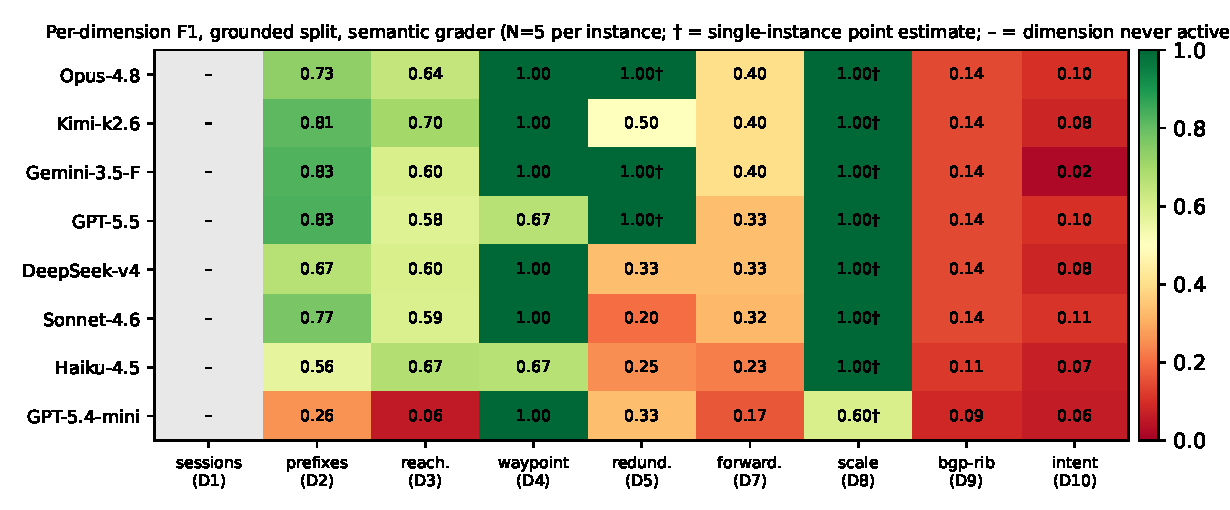
\includegraphics[width=\linewidth]{figs/fig_heatmap.pdf}
\caption{Per-dimension F1 on the grounded split (semantic grader), as
\emph{active-convention means}---precision and recall combined over every
instance where the dimension is active in truth or prediction. The
consequence-dimension cells (D7, D9, D10) are depressed by taxonomy-boundary
over-prediction, \emph{not} by missed detection: F1 where each is the
ground truth is high (Table~\ref{tab:grounded}, F3). The figure is shown to
expose that precision gap, not as a detection score.}
\label{fig:heatmap}
\end{figure}

\begin{figure}[t]
\centering
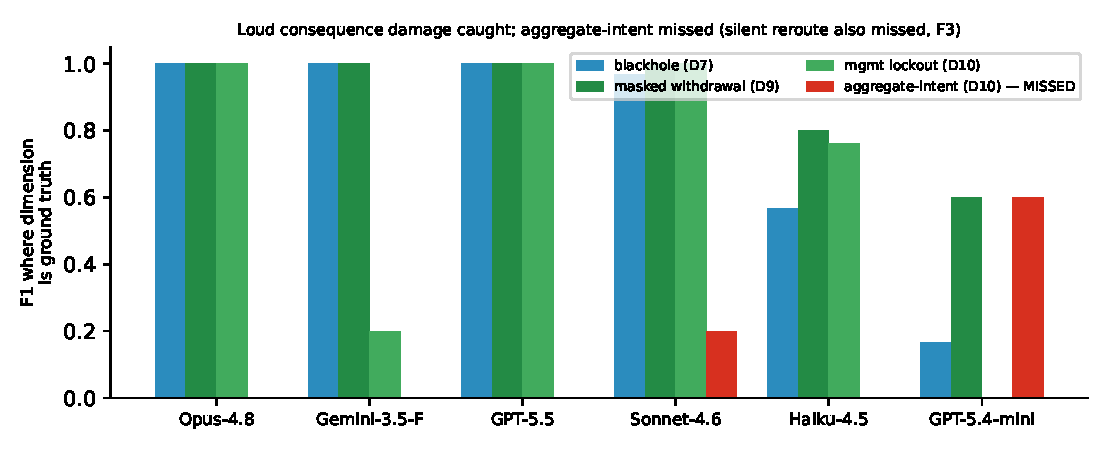
\includegraphics[width=0.85\linewidth]{figs/fig_gradient.pdf}
\caption{F1 where each consequence dimension is the ground truth
(grounded, semantic grader; on these single-truth instances F1 tracks
recall). The loud half---blackhole (D7), masked withdrawal (D9,
\emph{ipc3\_static}), management lockout (D10, \emph{mgmt\_lockout})---is
caught by the stronger models; the aggregate-preservation intent (D10,
\emph{ipc\_aggregate}) is missed. The sharpest quiet case, the leak-induced
silent reroute, is missed (F3) and is not plotted here.}
\label{fig:gradient}
\end{figure}

\paragraph{F1: The benchmark discriminates.} The eight models span
0.27--0.51 damage-detection macro-F1 on the grounded split: the four leaders
(Opus 4.8, Kimi k2.6, Gemini 3.5 Flash, GPT-5.5) cluster at 0.48--0.51, the
open-weight pair brackets the mid-tier (Kimi 0.49 tying the top of the fleet,
DeepSeek v4-pro 0.44 above both Sonnet 4.6 and Haiku 4.5), and GPT-5.4-mini
trails at 0.27; all model-free floors score $\leq$0.02 on that split
(Table~\ref{tab:grounded}). On the templated split's damage instances,
Haiku 4.5 and GPT-5.4-mini score 0.30$\pm$0.18 and 0.21$\pm$0.20 while the
modal-by-class memorizer scores \textbf{0.00} and the best other floor
0.075 (Figure~\ref{fig:floors}): the task is neither impossible nor
saturated, and performance is not explained by template recall.

\paragraph{F2: Models do not cry wolf on sessions.} The false-session-alarm
rate is 0.00 for every model on every split it was evaluated on---all 1{,}070
samples. The widely-assumed failure mode---hallucinating session losses on
any BGP-adjacent change---did not occur once, while the metric itself is
demonstrably sensitive (the strawman floor trips it at 1.00). Models do,
however, sometimes \emph{double-type} real damage: on silent-withdrawal
instances, models often report the dropped traffic both as reachability
loss (correct---the frontier scores 1.0 there on the very same samples) and
additionally as a forwarding anomaly---a typing the contract's own gloss
(``blackhole = no route'') invites but the oracle reserves for
discarded-while-routed flows. We charge these as false positives---and the
same taxonomy-boundary over-prediction extends to D9 and D10, where each
model labels a consequence dimension on roughly six and eight of the eleven
grounded instances the oracle reserves for a neighbor, depressing those
active-convention dimensional means (F3, Appendix~\ref{app:exact}) well
below the recall the models actually achieve where the dimension is the
truth. We flag the consequence-dimension boundaries for a sharpened v1.1
contract. On the empty-truth
calibration instances, the residual false alarms are sparse redundancy and
intent over-predictions by the two models evaluated on that split; no model
invents sessions, prefixes, or blackholes out of nothing.

\paragraph{F3: The blind spot is the quiet half, not the second order.}
We expected models to read first-order table effects and miss second-order
consequences. The data draw the line elsewhere. The \emph{loud} half is
read well across the fleet: five of the eight models---the four leaders plus
the open-weight DeepSeek v4-pro---identify both grounded blackholes on
every sample (10/10 each on \emph{leak\_ms} and \emph{clos\_summary}---the
latter a genuinely second-order, partial-ECMP consequence of a
summarization change), Sonnet 4.6 nearly matches them (D7 0.97), and
prefix-loss (D2) F1 is 0.67--0.83 across that group;
even the two cheapest models catch the explicit leak blackhole (Haiku 1.00
grounded, 0.98 on the templated leak-blackhole class), though they alone
miss the implicit, topology-emergent one (\emph{clos\_summary}: Haiku 0.13,
GPT-5.4-mini 0.13). Read where each
\emph{consequence} dimension is the ground truth, the picture is the same:
the masked control-plane withdrawal (\emph{ipc3\_static}, D9) is caught at
F1 1.00 by six models and 0.80/0.60 by the two cheapest; the
management-plane lockout (\emph{mgmt\_lockout}, D10) at 1.00 by Opus,
GPT-5.5, and Sonnet, 0.80 by both open-weight models (Haiku 0.76, Gemini
0.20); and the explicit LOCAL\_PREF waypoint bypass (\emph{lp\_waypoint},
D4) at 1.00 by all eight (Figure~\ref{fig:gradient}).

The \emph{quiet} half is the damage that survives this object-level
reading: reachability holds, and the harm is a path or policy the diff
never spells out. Its sharpest case is the leak-induced silent reroute, and
it \emph{separates the fleet} (Table~\ref{tab:reroute}). On the six reroute
instances---where a more-specific leak \emph{elsewhere} pulls a victim's
traffic past its mandated waypoint while the route still resolves and every
destination stays reachable---most models score zero on \emph{both} the
waypoint and intent dimensions on the majority of samples: GPT-5.4-mini and
Gemini 3.5 Flash on all 30, Haiku 4.5 on 27/30, Opus 4.8 on 21/30, and
Sonnet 4.6 on 18/30---and Opus and Gemini do this \emph{despite} topping the
loud half (their D7/D9/D10 are at or near 1.00). Only two models register it at
all: GPT-5.5 escapes total blindness on 29 of 30 samples (waypoint F1 0.64),
and the open-weight DeepSeek v4-pro on 20 of 30 (0.56)---and even these reads
are mostly of the waypoint \emph{element}; the paired traffic-pinning
\emph{intent} key is missed far more often (credited on 19/30 of GPT-5.5's
and 7/30 of DeepSeek's samples), so no model reliably reports the full
reroute. Reading the silent reroute is nonetheless a distinct capability
axis---uncorrelated with loud-half skill (Opus and Gemini top the loud half
yet miss the reroute) and not vendor-bound: a proprietary model (GPT-5.5)
and an open-weight one (DeepSeek) clear the field together (F4). This
differentiation is grader-dependent: under naive exact-string matching,
\emph{every} model scores both-zero on all 30 (the same probe-granularity
artifact as D7, \S\ref{sec:graderfinding}); the semantic grader's
canonicalization of the waypoint and intent keys is what exposes the split,
so the headline rests on the matching specification for D4/D10---config-derived
and floor-invariant (F5) but, unlike D1/D2/D8/D9, not provably the identity. A second, distinct quiet case is aggregate preservation: when a
customer's specific prefixes are dropped but a covering /24 survives
(\emph{ipc\_aggregate}), models catch the prefix loss (D2) yet miss the
traffic-pinning intent the surviving aggregate masks (D10 F1 $\leq$0.20 for
seven of the eight). The low \emph{dimensional} means for the consequence
dimensions (active-convention D7 0.17--0.40, D9 0.09--0.14, D10 0.02--0.11;
Figure~\ref{fig:heatmap}) are \emph{not} recall failures: they are dominated
by taxonomy-boundary false positives---each model predicts a consequence
dimension on roughly three (D7), six (D9), and eight (D10) of the eleven
grounded instances where the oracle reserves a neighboring label---the same
over-prediction the paper discloses for the D3/D7 boundary (F2). The genuine
miss is narrow and consistent: damage is read when it deletes or blackholes
something nameable, and missed---by most of the fleet---when every object
survives and only the path silently shifts. This is the path/policy-violation
kernel of the more-specific-leak class (the 2019 Cloudflare/Verizon leak among
them), which we model deterministically, isolated from the congestion and loss
the real incidents also produced (\S\ref{sec:task}). We measure the split on
six seed-and-scope variants of a \emph{single} leak-reroute mechanism; whether
it generalizes across structurally distinct quiet-reroute mechanisms---LOCAL\_PREF
steering, AS-path manipulation, aggregate masking---is the central open
question (\S\ref{sec:limitations}).

\begin{table}[t]
\centering\small
\begin{tabular}{@{}lcccc@{}}
\toprule
 & both-zero & waypoint & intent & waypoint \\
Model & (total miss) & credited & credited & F1 \\
\midrule
GPT-5.5                     & 1/30  & 29/30 & 19/30 & 0.64 \\
DeepSeek v4-pro \emph{(ow)} & 10/30 & 20/30 & 7/30  & 0.56 \\
Claude Sonnet 4.6           & 18/30 & 11/30 & 11/30 & 0.30 \\
Claude Opus 4.8             & 21/30 & 8/30  & 4/30  & 0.26 \\
Kimi k2.6 \emph{(ow)}       & \multicolumn{4}{c}{\textit{reroute run completing as of this draft}} \\
Claude Haiku 4.5            & 27/30 & 3/30  & 1/30  & 0.10 \\
GPT-5.4-mini                & 30/30 & 0/30  & 0/30  & 0.00 \\
Gemini 3.5 Flash            & 30/30 & 0/30  & 0/30  & 0.00 \\
\bottomrule
\end{tabular}
\caption{The silent reroute separates the fleet (six instances, $N{=}5$,
semantic grader). ``both-zero'' $=$ samples scoring 0 on \emph{both} the
waypoint (D4) and intent (D10) dimensions (total blindness); ``credited'' $=$
samples with nonzero F1 on that dimension. Two models clear the field
(GPT-5.5 and the open-weight DeepSeek), statistically tied at the top (paired
$t{=}1.3$, $n{=}6$ instances, n.s.) and well above the rest; the loud-half
leaders Opus 4.8 and Gemini 3.5 Flash miss it. Even the leaders credit the
traffic-pinning \emph{intent} key far less often than the waypoint element,
so no model reads the full reroute. Under exact-string matching every model
scores both-zero on all 30 (granularity artifact, \S\ref{sec:graderfinding});
the split is a semantic-grader result.}
\label{tab:reroute}
\end{table}

\paragraph{F4: No home-field advantage.} The benchmark was developed and
red-teamed primarily with Claude-family models, so grader circularity was a
live concern. Three lines of evidence rule it out. \emph{(i)~Frontier parity:}
the cross-vendor leaders land within noise of one another---Opus 4.8 at 0.51,
Kimi k2.6 at 0.49, Gemini 3.5 Flash at 0.49, GPT-5.5 at 0.48---a spread of
0.03 against a per-model standard error of $\approx$0.05 ($n{=}11$
instances), statistically indistinguishable (a Welch $t$-test on per-instance
means does not reject equality, $t{=}0.35$). \emph{(ii)~No Claude tilt:} the
second Anthropic model (Sonnet 4.6, 0.42) scores \emph{below} four
non-Anthropic models, and a non-Anthropic open-weight model (Kimi, 0.49)
ties the best non-Anthropic closed model, so the Claude-built benchmark does
not favor the Claude family. \emph{(iii)~On the headline:}
the one capability the benchmark most sharply discriminates---reading the
silent reroute (F3)---is cleared by two models, one proprietary (GPT-5.5) and
one \emph{open-weight} (DeepSeek v4-pro), statistically tied at the top
(paired $t{=}1.3$, $n{=}6$ instances, n.s.) and both well above the rest.
DeepSeek's waypoint F1 (0.56) exceeds every Anthropic and Google model's
(Opus 0.26, Sonnet 0.30, Haiku 0.10, Gemini 0.00)---significantly over Opus
(paired $t{=}2.7$, $p{=}0.045$) and marginally over the next-best Claude model
Sonnet ($t{=}2.2$, $p{=}0.08$, $n{=}6$). The robust statement is that an
open-weight reasoner stands among the two field-clearing models, so the
quiet-half gap is neither a Claude-family nor a closed-model artifact---though
on $n{=}6$ instances we do not claim a strict open-beats-all ordering.

\paragraph{F5: Naive set grading would have reported universal blindness.}
Under exact-string matching against the oracle's probe-granularity keys,
every model's active-convention forwarding-anomaly F1 is 0.00 (no
forwarding-anomaly-truth sample earns credit), and the
grounded frontier macro drops from 0.48--0.51 to 0.36--0.37
(Appendix~\ref{app:exact})---while the raw outputs contain the correct
node, kind, and config-visible prefix. The semantic canonicalization that
corrects this is provably the identity on the config-visible dimensions
(D1, D2, D8, D9) and leaves every model-free floor at chance (largest
movement: the syntactic-diff floor, 0.007$\to$0.023 templated), so the
correction lifts models, not floors---and only on the dimensions where the
raw outputs were right all along. We report this as a methods finding in its own
right: granularity-mismatched string grading is a silent way for a
verifier-graded benchmark to manufacture a dramatic, wrong headline.

\begin{figure}[t]
\centering
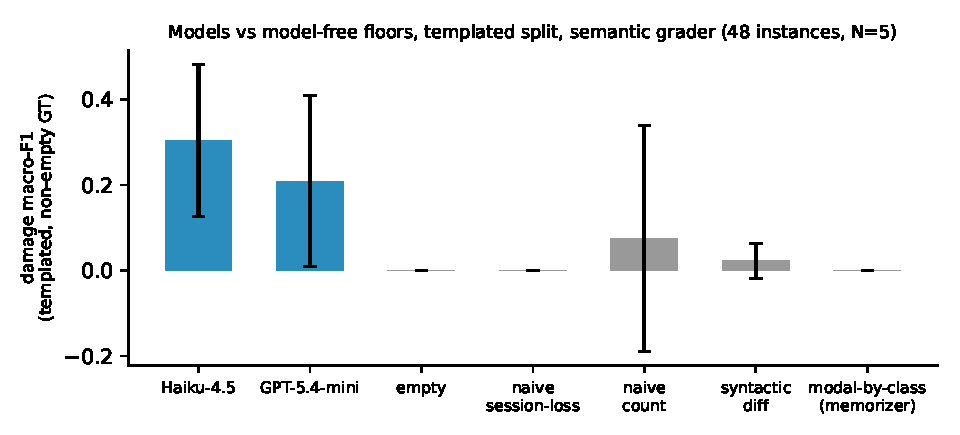
\includegraphics[width=0.85\linewidth]{figs/fig_floors.pdf}
\caption{Damage-detection macro-F1 versus model-free floors on the templated
split (semantic grader). The modal-by-class memorizer---the strongest
template-recall strategy---scores 0.00.}
\label{fig:floors}
\end{figure}

\section{Discussion}
\label{sec:discussion}

\paragraph{Why the quiet half matters most.} An assistant that misread
routing tables would be caught by any reviewer; an assistant that reads
them competently, catches the withdrawal and the lockout, never
false-alarms on sessions (F2), and yet silently misses the leak-induced
reroute (F3)---as most of the evaluated fleet does---is trusted exactly
where it is most dangerous---on the one failure mode that leaves no object
lost to catch. Binary safety metrics
cannot surface this: under a pass/fail rubric, a model that predicts
``no impact'' on a reroute instance is indistinguishable from one that
flags the waypoint bypass, because both made \emph{a} prediction. Typed,
graded affected-set scoring is what makes the quiet half measurable---and
the quiet half is where the most insidious incidents live: a leak that
reroutes a victim's traffic onto a path it should never take, with every
session up and every destination still reachable, exactly as in the 2019
route-leak outages.

\paragraph{A candidate graduation test for network agents.} As an
explicitly novel \emph{position} (a refinement orthogonal to TM~Forum's
autonomous-network levels), we propose blast-radius prediction as a
promotion gate on the autonomy ladder: \emph{advise}
$\rightarrow$ \emph{propose} $\rightarrow$ \emph{propose-with-self-check}
$\rightarrow$ \emph{gated-execute} $\rightarrow$ \emph{autonomous}---a
system would demonstrate, before advancing past \emph{propose}, that it can
enumerate the blast radius of its own changes at a calibrated
precision/recall point \emph{across all scored dimensions, including the
quiet ones}. No evaluated model fully meets that bar today, but the data
locate the frontier of the gate precisely. Every model passes on the loud
half of these 4--6 node networks; on the quiet half the strongest reasoners
are \emph{beginning} to pass---GPT-5.5 reads the silent reroute on 29 of 30
samples (waypoint F1 0.64) and the open-weight DeepSeek v4-pro on 20 of 30
(0.56)---while most of the fleet, including the models that top the loud
half (Opus 4.8, Gemini 3.5 Flash), still fails it outright. The gate
therefore discriminates twice: loud from quiet, and---within the quiet
half---the reasoning frontier from the rest, which is the kind of resolution
a promotion gate would need. We offer the autonomy ladder as a \emph{position},
not a validated instrument: establishing blast-radius prediction as an actual
gate requires the larger-topology and human-expert-baseline studies we defer
(\S\ref{sec:limitations}), and we conjecture---without testing it---that the
quiet-half gap does not close as topologies grow, since the inference chains
only lengthen.

\paragraph{Open problems.} Five follow directly. (1)~\emph{Tools-augmented
contrast}: how much of the quiet-half gap closes when the model may invoke
the verifier, and do agents invoke it on the changes that need it?
Cost-aware verifier invocation has been studied in general agentic
workflows~\cite{sherlock}; its networking instantiation---where a formal
oracle defines the invocation-policy optimum---is open, and Asadli et al.\
point at analyzing agents' tool-usage patterns as future
work~\cite{ethagentic}. (2)~\emph{Calibration}: are models
\emph{confidently} blind on the silent reroute, or do their confidences
flag the gap? (3)~\emph{Judge validity}: would an LLM-as-judge grader have
caught the granularity artifact of \S\ref{sec:graderfinding}, or introduced
its own? (4)~\emph{Learnability}: parameterized generators plus the oracle
yield unlimited perfectly-labeled training pairs; whether supervision
closes the quiet-half gap, or the gap survives infinite labels, is an open
empirical question. (5)~\emph{Contract sharpening}: the D3/D7 boundary
(F2) should be stated in the output contract precisely enough that
double-typing is unambiguous, without leaking the oracle's disposition
taxonomy.

\section{Related Work}
\label{sec:related}

The rapidly growing use of LLMs across network management and operations is
surveyed by Hong et al.~\cite{hong2025llmnetmgmt}; that survey catalogs intent
interpretation and task automation but does not treat pre-deployment safety
validation---the gap \netbrace{} targets.

\paragraph{LLM configuration synthesis and repair.} NetConfEval translates
intents into specifications and code~\cite{netconfeval}; Mondal et al.\
study LLM router-configuration synthesis with verifier
feedback~\cite{mondal}; PeeringLLM-Bench scores LLM synthesis of
vendor-specific {BGP} peering configurations from policy
intent~\cite{peeringllmbench}; CORNETTO benchmarks end-to-end
configuration repair
on 231 instances over real-world topologies of 20--754
nodes~\cite{cornetto}, and Asadli et al.\
show agentic architectures with retrieval and Batfish feedback improve
repair efficacy ($\sim$12\%) and reduce safety regressions
($\sim$17\%) over monolithic
prompting~\cite{ethagentic}, where the safety metric is a \emph{regression
score}: the fraction of the checked specification set that an
\emph{applied} fix newly breaks, computed by the verifier (lower is
better). \netbrace{} measures the complement: whether the \emph{model
itself}, with no verifier in the loop, can foresee typed damage from a diff.
The verifier is referee, not teammate.

\paragraph{Agentic network benchmarks.} NetArena (formerly NetPress)
generates dynamic agent tasks and scores correctness, latency, and a
rule-adherence action-safety axis in emulation~\cite{netarena};
NetAgentBench formalizes multi-turn configuration tasks as FSMs and
measures behavioral stability~\cite{netagentbench}; NIKA evaluates incident
diagnosis on emulated networks~\cite{nika}; the IRTF NMRG framework draft
defines NetConfBench, a 40-task emulator-based suite scored on
intent-achievement and functional correctness~\cite{nmrg}. Among these,
none scores an LLM's \emph{predicted} typed affected set---penalizing both
missed and hallucinated damage at the element level---from a static diff,
with no verifier in the model's loop. That conjunction is the gap
\netbrace{} fills.

\paragraph{Evaluation methodology.} Our design follows the rigor agenda for
agentic benchmarks~\cite{abc}: deterministic non-LLM grading, pinned
oracles, contamination controls, explicit floors, and multi-sample
reporting. The granularity pitfall of \S\ref{sec:graderfinding} is offered
as a concrete addition to that agenda. The holistic multi-metric framing
descends from HELM~\cite{helm}.

\section{Limitations}
\label{sec:limitations}

Single vendor dialect (FRR) and BGP-centric mechanisms in this release; the
packet-filter dimension (D6) is deferred pending a vendor dialect whose
ACLs Batfish models as interface filters. The D8 resource \emph{budget} is a
declared scenario parameter (the route count is computed; the limit is
spec'd, as platform limits are). Topologies are small (4--6 nodes), chosen
for oracle determinism; scale is untested, and while we see no mechanism by
which the quiet-half reasoning gap would \emph{close} as topologies grow,
that expectation is a conjecture, not a result. The grounded split is
11 scenarios; several dimensions appear there once and are reported as point
estimates, with the templated split carrying the statistics; the templated
split currently has no redundancy-truth (D5) instance, so templated D5
reflects only false-positive behavior. Evaluation is single-shot and
tool-free by design; agentic and tools-augmented conditions are the named
next step. Batfish models converged steady state, so transient and
timer-dependent damage is out of scope. Because grading is deterministic
set comparison against a pinned verifier, there is no human-judgment step
requiring inter-rater validation; the analogous validity question---does
the oracle compute the right ground truth?---is addressed by the
determinism gate, the live-FRR spot checks (\S\ref{sec:task}), and the
frozen matching specification. A human-\emph{expert baseline} (can a senior
operator enumerate the quiet half from the same evidence?) is the named
next experiment and is not claimed here---it is the load-bearing control for
reading the quiet-half miss as a \emph{model} limitation rather than intrinsic
task hardness. The headline silent-reroute result also rests on six
seed-and-scope variants of a \emph{single} leak-reroute mechanism; whether the
loud/quiet split generalizes to structurally distinct quiet-reroute mechanisms
(LOCAL\_PREF steering, AS-path manipulation, aggregate masking) is the central
open question and the first item a v1.1 must test. Relatedly, the reroute split
is a \emph{semantic-grader} result---under exact-string matching no model reads
it (F3)---so the matching specification for the flow-scoped dimensions D4/D7/D10
is a config-derived, floor-invariant, model-independent design choice (F5) that,
unlike the config-visible dimensions, has not been validated against independent
human judgments; a grader-validity check on those canonicalization decisions is
the natural complement to the human-expert baseline. The two open-weight models
were evaluated on the grounded and silent-reroute classes but not on the
cost-capped templated split, so their templated-floor comparison is deferred
with the full-fleet templated run.

\section{Conclusion}
\label{sec:conclusion}

We introduced typed blast-radius prediction, built an oracle-graded,
determinism-gated, judge-free benchmark for it, and measured where current
LLMs sit. The line we found is not the one we expected: models---including
mid-tier ones---catch the damage that announces itself, up to and including
a second-order partial-ECMP blackhole, and never hallucinate a session
loss; where most of them stumble---the one class that separates the
reasoning frontier from the rest---is the damage that removes no object and
only shifts the path: the leak-induced silent reroute past the inspection
node, where the route still resolves, the session stays up, and reachability
survives. Most of the fleet misses it even while catching the withdrawal,
the lockout, and the blackhole, which all delete something nameable; only
two models clear it---GPT-5.5 and the open-weight DeepSeek v4-pro, tied at the
top and well above the rest---an open-weight model standing among the
leaders, which rules out a closed-model or Claude-family artifact on the one
capability the benchmark most sharply discriminates. We
also showed how easily a verifier-graded benchmark can manufacture the
opposite, more dramatic headline through granularity-mismatched string
grading, and we release both graders with a frozen matching specification
so the correction is inspectable. Until the quiet half closes---or is
closed by verifier-in-the-loop architectures whose invocation policies are
themselves measured---LLM-proposed network changes need a blast-radius gate
that the proposing model cannot currently pass on exactly the failures that
matter most. The benchmark, oracle pipeline, run artifacts, and floors make
that gate, and progress against it, measurable.

\paragraph{Artifacts.} Code, scenario suites, generator seeds, pinned
oracle digests, determinism reports, prompts, raw model outputs, graded
results under both graders, and the frozen semantic-matching specification
will be released alongside the peer-reviewed version; every number in this
report traces to a saved run artifact (including the pooled Gemini sample
set, both Sonnet runs, and the eight-model silent-reroute extension) and will
be reproducible from that release.

\paragraph{Acknowledgments and AI disclosure.} LLM tooling (Claude) was
used extensively under the author's direction for drafting, engineering,
and analysis, including adversarial review passes that surfaced the grading
artifact reported in \S\ref{sec:graderfinding}. All experiments, numbers,
and citations were verified by the author, who takes sole responsibility
for the content.

\appendix

\section{Exact-string grading: the conservative lower bound}
\label{app:exact}

Table~\ref{tab:exact} reports the grounded split under both graders. The
exact-string grader demands byte-identical element keys, including the
oracle's undisclosed probe-/32 destinations on flow-scoped dimensions; the
semantic grader (\S\ref{sec:grading}) canonicalizes probes to
config-visible covers under a frozen, floor-invariant specification.
Dimensions whose truth is already config-visible (D1, D2, D8, D9) are
provably identical under both graders, as is the false-session-alarm
metric.

\begin{table}[h]
\centering\small
\begin{tabular}{@{}lcccc@{}}
\toprule
 & \multicolumn{2}{c}{macro-F1 (damage)} & \multicolumn{2}{c}{forwarding D7 (active conv.)} \\
Model & exact & semantic & exact & semantic \\
\midrule
Claude Opus 4.8       & 0.37$\pm$0.27 & 0.51$\pm$0.17 & 0.00 & 0.40 \\
Kimi k2.6 \emph{(ow)} & 0.36$\pm$0.24 & 0.49$\pm$0.12 & 0.00 & 0.40 \\
Gemini 3.5 Flash      & 0.36$\pm$0.28 & 0.49$\pm$0.18 & 0.00 & 0.40 \\
GPT-5.5               & 0.36$\pm$0.27 & 0.48$\pm$0.17 & 0.00 & 0.33 \\
DeepSeek v4-pro \emph{(ow)} & 0.31$\pm$0.18 & 0.44$\pm$0.08 & 0.00 & 0.33 \\
Claude Sonnet 4.6     & 0.30$\pm$0.17 & 0.42$\pm$0.06 & 0.00 & 0.32 \\
Claude Haiku 4.5      & 0.29$\pm$0.17 & 0.39$\pm$0.10 & 0.00 & 0.23 \\
GPT-5.4-mini          & 0.22$\pm$0.22 & 0.27$\pm$0.21 & 0.00 & 0.17 \\
\bottomrule
\end{tabular}
\caption{Grounded split under both graders. The exact-string D7 column is
0.00 for every model on every forwarding-anomaly-truth sample---the granularity artifact of
\S\ref{sec:graderfinding}. The semantic D7 column uses the
active-instance convention and is depressed below the anomaly-truth
recall of Table~\ref{tab:grounded} by the D3/D7 double-typing false
positives discussed in F2. Sonnet's grounded rows are from the
12{,}000-token re-run (Disclosure ii); the exact-string column moves it
from 0.30 to 0.42 under semantic matching, the same lift seen fleet-wide.
}
\label{tab:exact}
\end{table}

\begin{thebibliography}{15}\small

\bibitem{ethagentic}
R.~Asadli, B.~Hoffman, I.~Protogeros, and L.~Vanbever.
\newblock Evaluating agentic configuration repair for computer networks.
\newblock arXiv:2606.06212, 2026.

\bibitem{cornetto}
I.~Protogeros, R.~Asadli, B.~Hoffman, and L.~Vanbever.
\newblock Benchmarking {LLM}-driven network configuration repair.
\newblock arXiv:2604.22513, 2026.

\bibitem{netarena}
Y.~Zhou, J.~Ruan, E.~Wang, S.~Fouladi, F.~Y. Yan, K.~Hsieh, and Z.~Liu.
\newblock {NetArena}: Dynamic benchmarks for {AI} agents in network
automation.
\newblock In \emph{Proc.\ ICLR}, 2026. arXiv:2506.03231 (v1 titled
\emph{NetPress}, 2025).

\bibitem{netagentbench}
A.~Twabi, Y.~Ding, and T.~Kondo.
\newblock {NetAgentBench}: A state-centric benchmark for evaluating agentic
network configuration.
\newblock arXiv:2604.09678, 2026.

\bibitem{nika}
Z.~Wang, A.~Cornacchia, A.~Sacco, F.~Galante, M.~Canini, and D.~Jiang.
\newblock {NIKA}: A network arena for benchmarking {AI} agents on network
troubleshooting.
\newblock arXiv:2512.16381, 2025.

\bibitem{netconfeval}
C.~Wang, M.~Scazzariello, A.~Farshin, S.~Ferlin, D.~Kosti\'c, and
M.~Chiesa.
\newblock {NetConfEval}: Can {LLMs} facilitate network configuration?
\newblock In \emph{Proc.\ ACM CoNEXT}, 2024. arXiv:2309.06342.

\bibitem{mondal}
R.~Mondal, A.~Tang, R.~Beckett, T.~Millstein, and G.~Varghese.
\newblock What do {LLMs} need to synthesize correct router configurations?
\newblock In \emph{Proc.\ ACM HotNets}, 2023. arXiv:2307.04945.

\bibitem{peeringllmbench}
J.~R.~Mendoza and R.~Ocampo.
\newblock {PeeringLLM-Bench}: Evaluating {LLMs} for {BGP} configuration tasks.
\newblock In \emph{Proc.\ 20th Asian Internet Engineering Conf.\ (AINTEC)},
2025. DOI:10.1145/3763400.3763451.

\bibitem{hong2025llmnetmgmt}
J.~Hong, N.~V.~Tu, and J.~W.-K. Hong.
\newblock A comprehensive survey on {LLM}-based network management and
operations.
\newblock \emph{Int.\ J.\ Network Management}, 35(6):e70029, 2025.
DOI:10.1002/nem.70029.

\bibitem{nmrg}
Y.~Cui et al.
\newblock A framework for {LLM} benchmarking in network configuration
({NetConfBench}).
\newblock IRTF Network Management Research Group, Internet-Draft
draft-cui-nmrg-llm-benchmark-01, December 2025.

\bibitem{batfish}
A.~Fogel, S.~Fung, L.~Pedrosa, M.~Walraed-Sullivan, R.~Govindan,
R.~Mahajan, and T.~Millstein.
\newblock A general approach to network configuration analysis.
\newblock In \emph{Proc.\ USENIX NSDI}, 2015.

\bibitem{rfc7938}
P.~Lapukhov, A.~Premji, and J.~Mitchell.
\newblock Use of {BGP} for routing in large-scale data centers.
\newblock RFC 7938, IETF, August 2016.

\bibitem{sherlock}
Y.~Ro, H.~Qiu, I.~Goiri, R.~Fonseca, R.~Bianchini, A.~Akella, Z.~Wang,
M.~Erez, and E.~Choukse.
\newblock Sherlock: Reliable and efficient agentic workflow execution.
\newblock arXiv:2511.00330, 2025.

\bibitem{abc}
Zhu et al.
\newblock Establishing best practices for building rigorous agentic
benchmarks.
\newblock arXiv:2507.02825, 2025.

\bibitem{helm}
P.~Liang et al.
\newblock Holistic evaluation of language models.
\newblock \emph{Transactions on Machine Learning Research}, 2023.
arXiv:2211.09110.

\end{thebibliography}

\end{document}
